\subsection{Startup behavior of the ozone generator}
\label{sec:ozone}

During these first experiments, I wanted to assure that the ozone
generator produces enough ozone. More precisely I was interested,
whether the ozone could penetrate the silica gel and how long it would
take for it to succeed. In a last step, I wanted to roughly estimate
the relation between the ozone production and the applied electrical
current at the mercury lamp.

\subsubsection{Setup}
\label{sec:ozone-setup}

The following experiments were all conducted using the setup described
in Section~\ref{sec:ozone-setup}. Since the cuvette had to be entered
in and removed from the lightpath manually, the time resolution had to
be reduced to \SI{5}{\minute}. In a first step, I measured the startup
\ch{O3} transmission through the silica gel filter after a one week
stop of the generator. Secondly, I researched the startup time
necessary after shorter stops. Lastly, I noted the influence of the
lamp current on the ozone concentration. Using this setup it was
impossible to measure the generator's \ch{NO2} production. Since the
concentration should be around the \ch{NO_x} concentration in ambient
lab air, it should be no more than a few \si{ppb}. This is far below
the detection limit of a `Longpath'-DOAS instrument with a pathlength
of \SI{8.6}{\centi\meter} and a LED peak at $\lambda \approx
\SI{290}{\nano\meter}$.

\subsubsection{Results}
\label{sec:ozone-results}

As a zeroth, qualitative experiment I turned on the generator
and succeeded in perceiving an ozone signal. After that I shut down the generator
for one week. The startup behavior afterwards can be seen in
Figure~\ref{fig:long-stop}. It shows that the generator takes about
\SI{35}{\minute} before it reaches its stable plateau of around
\SI{250}{ppb} ozone. During this experiment the flow was constantly
set to $\Phi_{\ch{O_3}} = \SI{0.03}{\liter\per\minute}$. It stands to
argue that the startup time could be shortened by increasing the flow,
however, as shall be seen shortly, if the
generator is used regularly, this procedure seems unnecessary.

\begin{figure}[htbp]
  \centering
  % GNUPLOT: LaTeX picture with Postscript
\begingroup
  \makeatletter
  \providecommand\color[2][]{%
    \GenericError{(gnuplot) \space\space\space\@spaces}{%
      Package color not loaded in conjunction with
      terminal option `colourtext'%
    }{See the gnuplot documentation for explanation.%
    }{Either use 'blacktext' in gnuplot or load the package
      color.sty in LaTeX.}%
    \renewcommand\color[2][]{}%
  }%
  \providecommand\includegraphics[2][]{%
    \GenericError{(gnuplot) \space\space\space\@spaces}{%
      Package graphicx or graphics not loaded%
    }{See the gnuplot documentation for explanation.%
    }{The gnuplot epslatex terminal needs graphicx.sty or graphics.sty.}%
    \renewcommand\includegraphics[2][]{}%
  }%
  \providecommand\rotatebox[2]{#2}%
  \@ifundefined{ifGPcolor}{%
    \newif\ifGPcolor
    \GPcolorfalse
  }{}%
  \@ifundefined{ifGPblacktext}{%
    \newif\ifGPblacktext
    \GPblacktexttrue
  }{}%
  % define a \g@addto@macro without @ in the name:
  \let\gplgaddtomacro\g@addto@macro
  % define empty templates for all commands taking text:
  \gdef\gplbacktext{}%
  \gdef\gplfronttext{}%
  \makeatother
  \ifGPblacktext
    % no textcolor at all
    \def\colorrgb#1{}%
    \def\colorgray#1{}%
  \else
    % gray or color?
    \ifGPcolor
      \def\colorrgb#1{\color[rgb]{#1}}%
      \def\colorgray#1{\color[gray]{#1}}%
      \expandafter\def\csname LTw\endcsname{\color{white}}%
      \expandafter\def\csname LTb\endcsname{\color{black}}%
      \expandafter\def\csname LTa\endcsname{\color{black}}%
      \expandafter\def\csname LT0\endcsname{\color[rgb]{1,0,0}}%
      \expandafter\def\csname LT1\endcsname{\color[rgb]{0,1,0}}%
      \expandafter\def\csname LT2\endcsname{\color[rgb]{0,0,1}}%
      \expandafter\def\csname LT3\endcsname{\color[rgb]{1,0,1}}%
      \expandafter\def\csname LT4\endcsname{\color[rgb]{0,1,1}}%
      \expandafter\def\csname LT5\endcsname{\color[rgb]{1,1,0}}%
      \expandafter\def\csname LT6\endcsname{\color[rgb]{0,0,0}}%
      \expandafter\def\csname LT7\endcsname{\color[rgb]{1,0.3,0}}%
      \expandafter\def\csname LT8\endcsname{\color[rgb]{0.5,0.5,0.5}}%
    \else
      % gray
      \def\colorrgb#1{\color{black}}%
      \def\colorgray#1{\color[gray]{#1}}%
      \expandafter\def\csname LTw\endcsname{\color{white}}%
      \expandafter\def\csname LTb\endcsname{\color{black}}%
      \expandafter\def\csname LTa\endcsname{\color{black}}%
      \expandafter\def\csname LT0\endcsname{\color{black}}%
      \expandafter\def\csname LT1\endcsname{\color{black}}%
      \expandafter\def\csname LT2\endcsname{\color{black}}%
      \expandafter\def\csname LT3\endcsname{\color{black}}%
      \expandafter\def\csname LT4\endcsname{\color{black}}%
      \expandafter\def\csname LT5\endcsname{\color{black}}%
      \expandafter\def\csname LT6\endcsname{\color{black}}%
      \expandafter\def\csname LT7\endcsname{\color{black}}%
      \expandafter\def\csname LT8\endcsname{\color{black}}%
    \fi
  \fi
    \setlength{\unitlength}{0.0500bp}%
    \ifx\gptboxheight\undefined%
      \newlength{\gptboxheight}%
      \newlength{\gptboxwidth}%
      \newsavebox{\gptboxtext}%
    \fi%
    \setlength{\fboxrule}{0.5pt}%
    \setlength{\fboxsep}{1pt}%
\begin{picture}(7776.00,3888.00)%
    \gplgaddtomacro\gplbacktext{%
      \csname LTb\endcsname%
      \put(814,704){\makebox(0,0)[r]{\strut{}$0$}}%
      \put(814,1191){\makebox(0,0)[r]{\strut{}$50$}}%
      \put(814,1677){\makebox(0,0)[r]{\strut{}$100$}}%
      \put(814,2164){\makebox(0,0)[r]{\strut{}$150$}}%
      \put(814,2650){\makebox(0,0)[r]{\strut{}$200$}}%
      \put(814,3137){\makebox(0,0)[r]{\strut{}$250$}}%
      \put(814,3623){\makebox(0,0)[r]{\strut{}$300$}}%
      \put(946,484){\makebox(0,0){\strut{}$0$}}%
      \put(2233,484){\makebox(0,0){\strut{}$0.5$}}%
      \put(3519,484){\makebox(0,0){\strut{}$1$}}%
      \put(4806,484){\makebox(0,0){\strut{}$1.5$}}%
      \put(6092,484){\makebox(0,0){\strut{}$2$}}%
      \put(7379,484){\makebox(0,0){\strut{}$2.5$}}%
    }%
    \gplgaddtomacro\gplfronttext{%
      \csname LTb\endcsname%
      \put(176,2163){\rotatebox{-270}{\makebox(0,0){\strut{}Concentration [ppm]}}}%
      \put(4162,154){\makebox(0,0){\strut{}Time [h]}}%
    }%
    \gplbacktext
    \put(0,0){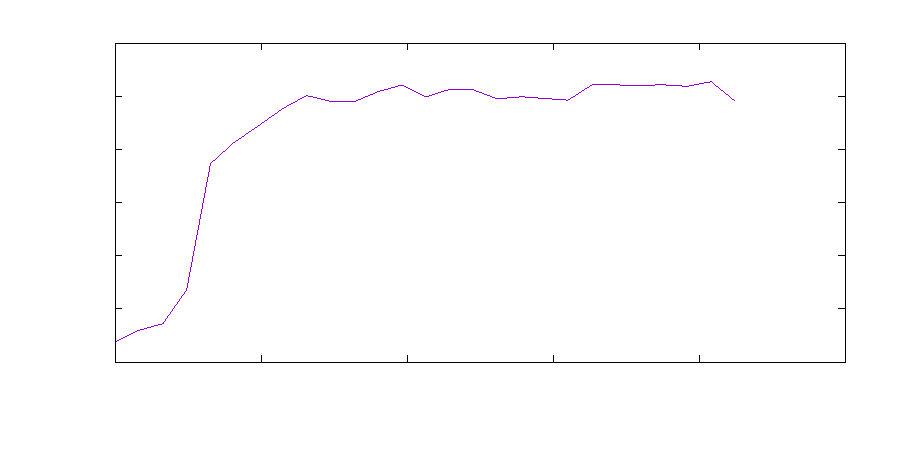
\includegraphics{../images/startup}}%
    \gplfronttext
  \end{picture}%
\endgroup

  \caption{Evolution of ozone after a long (one week) full stop of the
    generator.}
  \label{fig:long-stop}
\end{figure}
\begin{figure}[htbp]
  \centering
  % GNUPLOT: LaTeX picture with Postscript
\begingroup
  \makeatletter
  \providecommand\color[2][]{%
    \GenericError{(gnuplot) \space\space\space\@spaces}{%
      Package color not loaded in conjunction with
      terminal option `colourtext'%
    }{See the gnuplot documentation for explanation.%
    }{Either use 'blacktext' in gnuplot or load the package
      color.sty in LaTeX.}%
    \renewcommand\color[2][]{}%
  }%
  \providecommand\includegraphics[2][]{%
    \GenericError{(gnuplot) \space\space\space\@spaces}{%
      Package graphicx or graphics not loaded%
    }{See the gnuplot documentation for explanation.%
    }{The gnuplot epslatex terminal needs graphicx.sty or graphics.sty.}%
    \renewcommand\includegraphics[2][]{}%
  }%
  \providecommand\rotatebox[2]{#2}%
  \@ifundefined{ifGPcolor}{%
    \newif\ifGPcolor
    \GPcolorfalse
  }{}%
  \@ifundefined{ifGPblacktext}{%
    \newif\ifGPblacktext
    \GPblacktexttrue
  }{}%
  % define a \g@addto@macro without @ in the name:
  \let\gplgaddtomacro\g@addto@macro
  % define empty templates for all commands taking text:
  \gdef\gplbacktext{}%
  \gdef\gplfronttext{}%
  \makeatother
  \ifGPblacktext
    % no textcolor at all
    \def\colorrgb#1{}%
    \def\colorgray#1{}%
  \else
    % gray or color?
    \ifGPcolor
      \def\colorrgb#1{\color[rgb]{#1}}%
      \def\colorgray#1{\color[gray]{#1}}%
      \expandafter\def\csname LTw\endcsname{\color{white}}%
      \expandafter\def\csname LTb\endcsname{\color{black}}%
      \expandafter\def\csname LTa\endcsname{\color{black}}%
      \expandafter\def\csname LT0\endcsname{\color[rgb]{1,0,0}}%
      \expandafter\def\csname LT1\endcsname{\color[rgb]{0,1,0}}%
      \expandafter\def\csname LT2\endcsname{\color[rgb]{0,0,1}}%
      \expandafter\def\csname LT3\endcsname{\color[rgb]{1,0,1}}%
      \expandafter\def\csname LT4\endcsname{\color[rgb]{0,1,1}}%
      \expandafter\def\csname LT5\endcsname{\color[rgb]{1,1,0}}%
      \expandafter\def\csname LT6\endcsname{\color[rgb]{0,0,0}}%
      \expandafter\def\csname LT7\endcsname{\color[rgb]{1,0.3,0}}%
      \expandafter\def\csname LT8\endcsname{\color[rgb]{0.5,0.5,0.5}}%
    \else
      % gray
      \def\colorrgb#1{\color{black}}%
      \def\colorgray#1{\color[gray]{#1}}%
      \expandafter\def\csname LTw\endcsname{\color{white}}%
      \expandafter\def\csname LTb\endcsname{\color{black}}%
      \expandafter\def\csname LTa\endcsname{\color{black}}%
      \expandafter\def\csname LT0\endcsname{\color{black}}%
      \expandafter\def\csname LT1\endcsname{\color{black}}%
      \expandafter\def\csname LT2\endcsname{\color{black}}%
      \expandafter\def\csname LT3\endcsname{\color{black}}%
      \expandafter\def\csname LT4\endcsname{\color{black}}%
      \expandafter\def\csname LT5\endcsname{\color{black}}%
      \expandafter\def\csname LT6\endcsname{\color{black}}%
      \expandafter\def\csname LT7\endcsname{\color{black}}%
      \expandafter\def\csname LT8\endcsname{\color{black}}%
    \fi
  \fi
    \setlength{\unitlength}{0.0500bp}%
    \ifx\gptboxheight\undefined%
      \newlength{\gptboxheight}%
      \newlength{\gptboxwidth}%
      \newsavebox{\gptboxtext}%
    \fi%
    \setlength{\fboxrule}{0.5pt}%
    \setlength{\fboxsep}{1pt}%
\begin{picture}(4030.00,4030.00)%
    \gplgaddtomacro\gplbacktext{%
      \csname LTb\endcsname%
      \put(814,704){\makebox(0,0)[r]{\strut{}$80$}}%
      \put(814,1141){\makebox(0,0)[r]{\strut{}$100$}}%
      \put(814,1579){\makebox(0,0)[r]{\strut{}$120$}}%
      \put(814,2016){\makebox(0,0)[r]{\strut{}$140$}}%
      \put(814,2453){\makebox(0,0)[r]{\strut{}$160$}}%
      \put(814,2890){\makebox(0,0)[r]{\strut{}$180$}}%
      \put(814,3328){\makebox(0,0)[r]{\strut{}$200$}}%
      \put(814,3765){\makebox(0,0)[r]{\strut{}$220$}}%
      \put(946,484){\makebox(0,0){\strut{}$0$}}%
      \put(1483,484){\makebox(0,0){\strut{}$2$}}%
      \put(2021,484){\makebox(0,0){\strut{}$4$}}%
      \put(2558,484){\makebox(0,0){\strut{}$6$}}%
      \put(3096,484){\makebox(0,0){\strut{}$8$}}%
      \put(3633,484){\makebox(0,0){\strut{}$10$}}%
    }%
    \gplgaddtomacro\gplfronttext{%
      \csname LTb\endcsname%
      \put(176,2234){\rotatebox{-270}{\makebox(0,0){\strut{}Concentration [ppm]}}}%
      \put(2289,154){\makebox(0,0){\strut{}Time [min]}}%
      \csname LTb\endcsname%
      \put(2646,1537){\makebox(-200,0){\nfrac{} 1/2 h}}%
      \csname LTb\endcsname%
      \put(2646,1317){\makebox(-100,0){1 h}}%
      \csname LTb\endcsname%
      \put(2646,1097){\makebox(-100,0){2 h}}%
      \csname LTb\endcsname%
      \put(2646,877){\makebox(-100,0){4 h}}%
    }%
    \gplbacktext
    \put(0,0){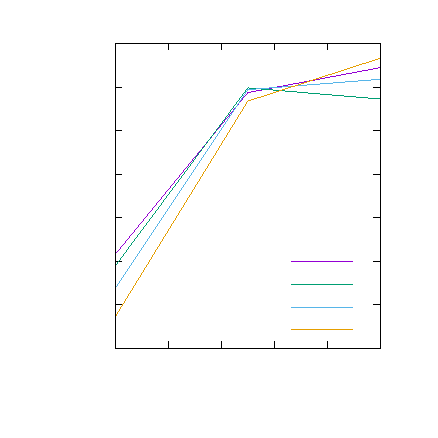
\includegraphics{../images/multi}}%
    \gplfronttext
  \end{picture}%
\endgroup

  \hfill
  % GNUPLOT: LaTeX picture with Postscript
\begingroup
  \makeatletter
  \providecommand\color[2][]{%
    \GenericError{(gnuplot) \space\space\space\@spaces}{%
      Package color not loaded in conjunction with
      terminal option `colourtext'%
    }{See the gnuplot documentation for explanation.%
    }{Either use 'blacktext' in gnuplot or load the package
      color.sty in LaTeX.}%
    \renewcommand\color[2][]{}%
  }%
  \providecommand\includegraphics[2][]{%
    \GenericError{(gnuplot) \space\space\space\@spaces}{%
      Package graphicx or graphics not loaded%
    }{See the gnuplot documentation for explanation.%
    }{The gnuplot epslatex terminal needs graphicx.sty or graphics.sty.}%
    \renewcommand\includegraphics[2][]{}%
  }%
  \providecommand\rotatebox[2]{#2}%
  \@ifundefined{ifGPcolor}{%
    \newif\ifGPcolor
    \GPcolorfalse
  }{}%
  \@ifundefined{ifGPblacktext}{%
    \newif\ifGPblacktext
    \GPblacktexttrue
  }{}%
  % define a \g@addto@macro without @ in the name:
  \let\gplgaddtomacro\g@addto@macro
  % define empty templates for all commands taking text:
  \gdef\gplbacktext{}%
  \gdef\gplfronttext{}%
  \makeatother
  \ifGPblacktext
    % no textcolor at all
    \def\colorrgb#1{}%
    \def\colorgray#1{}%
  \else
    % gray or color?
    \ifGPcolor
      \def\colorrgb#1{\color[rgb]{#1}}%
      \def\colorgray#1{\color[gray]{#1}}%
      \expandafter\def\csname LTw\endcsname{\color{white}}%
      \expandafter\def\csname LTb\endcsname{\color{black}}%
      \expandafter\def\csname LTa\endcsname{\color{black}}%
      \expandafter\def\csname LT0\endcsname{\color[rgb]{1,0,0}}%
      \expandafter\def\csname LT1\endcsname{\color[rgb]{0,1,0}}%
      \expandafter\def\csname LT2\endcsname{\color[rgb]{0,0,1}}%
      \expandafter\def\csname LT3\endcsname{\color[rgb]{1,0,1}}%
      \expandafter\def\csname LT4\endcsname{\color[rgb]{0,1,1}}%
      \expandafter\def\csname LT5\endcsname{\color[rgb]{1,1,0}}%
      \expandafter\def\csname LT6\endcsname{\color[rgb]{0,0,0}}%
      \expandafter\def\csname LT7\endcsname{\color[rgb]{1,0.3,0}}%
      \expandafter\def\csname LT8\endcsname{\color[rgb]{0.5,0.5,0.5}}%
    \else
      % gray
      \def\colorrgb#1{\color{black}}%
      \def\colorgray#1{\color[gray]{#1}}%
      \expandafter\def\csname LTw\endcsname{\color{white}}%
      \expandafter\def\csname LTb\endcsname{\color{black}}%
      \expandafter\def\csname LTa\endcsname{\color{black}}%
      \expandafter\def\csname LT0\endcsname{\color{black}}%
      \expandafter\def\csname LT1\endcsname{\color{black}}%
      \expandafter\def\csname LT2\endcsname{\color{black}}%
      \expandafter\def\csname LT3\endcsname{\color{black}}%
      \expandafter\def\csname LT4\endcsname{\color{black}}%
      \expandafter\def\csname LT5\endcsname{\color{black}}%
      \expandafter\def\csname LT6\endcsname{\color{black}}%
      \expandafter\def\csname LT7\endcsname{\color{black}}%
      \expandafter\def\csname LT8\endcsname{\color{black}}%
    \fi
  \fi
    \setlength{\unitlength}{0.0500bp}%
    \ifx\gptboxheight\undefined%
      \newlength{\gptboxheight}%
      \newlength{\gptboxwidth}%
      \newsavebox{\gptboxtext}%
    \fi%
    \setlength{\fboxrule}{0.5pt}%
    \setlength{\fboxsep}{1pt}%
\begin{picture}(4030.00,4030.00)%
    \gplgaddtomacro\gplbacktext{%
      \csname LTb\endcsname%
      \put(814,704){\makebox(0,0)[r]{\strut{}$200$}}%
      \put(814,1010){\makebox(0,0)[r]{\strut{}$220$}}%
      \put(814,1316){\makebox(0,0)[r]{\strut{}$240$}}%
      \put(814,1622){\makebox(0,0)[r]{\strut{}$260$}}%
      \put(814,1928){\makebox(0,0)[r]{\strut{}$280$}}%
      \put(814,2235){\makebox(0,0)[r]{\strut{}$300$}}%
      \put(814,2541){\makebox(0,0)[r]{\strut{}$320$}}%
      \put(814,2847){\makebox(0,0)[r]{\strut{}$340$}}%
      \put(814,3153){\makebox(0,0)[r]{\strut{}$360$}}%
      \put(814,3459){\makebox(0,0)[r]{\strut{}$380$}}%
      \put(814,3765){\makebox(0,0)[r]{\strut{}$400$}}%
      \put(946,484){\makebox(0,0){\strut{}$0$}}%
      \put(1245,484){\makebox(0,0){\strut{}$5$}}%
      \put(1543,484){\makebox(0,0){\strut{}$10$}}%
      \put(1842,484){\makebox(0,0){\strut{}$15$}}%
      \put(2140,484){\makebox(0,0){\strut{}$20$}}%
      \put(2439,484){\makebox(0,0){\strut{}$25$}}%
      \put(2737,484){\makebox(0,0){\strut{}$30$}}%
      \put(3036,484){\makebox(0,0){\strut{}$35$}}%
      \put(3334,484){\makebox(0,0){\strut{}$40$}}%
      \put(3633,484){\makebox(0,0){\strut{}$45$}}%
    }%
    \gplgaddtomacro\gplfronttext{%
      \csname LTb\endcsname%
      \put(176,2234){\rotatebox{-270}{\makebox(0,0){\strut{}Concentration [ppm]}}}%
      \put(2289,154){\makebox(0,0){\strut{}Time [min]}}%
    }%
    \gplbacktext
    \put(0,0){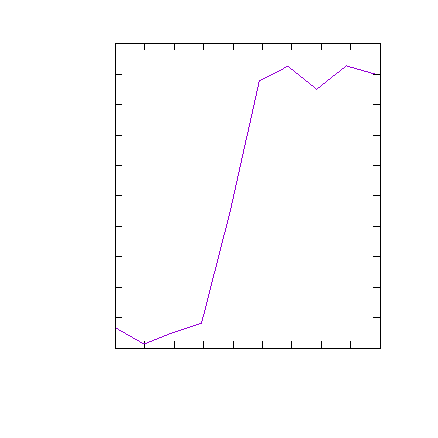
\includegraphics{../images/current}}%
    \gplfronttext
  \end{picture}%
\endgroup

  \caption{Left: Evolution of the ozone concentration after a full stop of the
    generator for different waiting times. Right: Ozone level
    dependence on the current of the mercury lamp. The steep
    flank occurred after a change of the current from
    \SI{10}{\milli\ampere} to \SI{17}{\milli\ampere}.}
  \label{fig:multiple-stop}
\end{figure}

After determining the longtime behavior, I was interested in
short term pauses. For that reason I stopped the generator (after it
had stabilized) for {\nfrac{} 1/2} \si{\hour}, \SI{1}{\hour},
\SI{2}{\hour} and \SI{4}{\hour} and measured the startup time. The
result can be found in Figure~\ref{fig:multiple-stop}
left-hand side. Since the time resolution of the DOAS instrument is
rather coarse, the only safe statement is that even after a
\SI{4}{\hour} stop the concentration climbed back up to around
\SI{200}{ppb} after \SI{5}{\minute}. So it stands to reason, that if
the device is used regularly a prolonged startup time should not be an
issue, even if one sticks to the constant flow of $\Phi_{\ch{O3}} =
\SI{0.03}{\liter\per\minute}$.

As compared to the ozone level in Figure~\ref{fig:long-stop}, the
plateau seems to lie slightly lower in this second experiment. The
reason for this lies most probably in the stabilization of the mercury
lamp, which was factory new during the first measurements.

After having analyzed the startup procedure, I wanted to investigate
the qualitative influence of the power supply current of the mercury
lamp on the ozone concentration. Beforehand it was not clear whether a
higher current would increase or decrease the ozone production rate,
as I did not know how a change in power would transform the power
distribution of the different mercury lines (c.\,f.\
Sec.~\ref{sec:theory-ozone}). I recorded a time series while switching
between the two possible currents, \SI{10}{\milli\ampere} and
\SI{17}{\milli\ampere}, and obtained Figure~\ref{fig:multiple-stop}
right-hand side. From this one can see that the generator still works
in a regime where a higher current leads to more ozone. However, this
fact is secondary in nature for my purposes, as I do not wish to
maximize the ozone output. \SI{200}{ppm} ozone allows for the
minimization of the ozone generator flow entering the sample air
stream, minimizing the effects due to dilution, while still supplying
enough ozone for the conversion. Thus any ozone concentration in this
region is well suited for my purposes. Hence I always applied the
preset current to the mercury lamp.

%%% Local Variables: 
%%% mode: latex
%%% TeX-master: "../Bachelor"
%%% End: 
